\PassOptionsToPackage{hyphens}{url}
\documentclass[compress,aspectratio=169]{beamer}
\usepackage{enumitem}

\usetheme{Goettingen}

\graphicspath{{../2019-06-isc/}{../2019-06-isc/fig/}{./fig/}{../logo/}}

\newcommand{\ok}[1]{{#1 (done)}}
\newcommand{\ongoing}[1]{{#1 (ongoing)}}
\newcommand{\started}[1]{{#1 (started)}}
\newcommand{\pending}[1]{{#1 (pending in plan)}}
\newcommand{\hrefb}[2]{\href{#1}{\textcolor{blue}{#2}}}

\subtitle{}
\title{\Large Benefit for utilizing HPC CF - Partiticipation of the TU Dresden}
\author{Anja Gerbes}
\date{2023-05-23}
\authorURL{https://hpc-certification.org}
\authorFooter{Julian M. Kunkel et al.}
\venue{ISC 23 BoF}
\institute{Technische Universität Dresden, ZIH }
\groupLogo{
\includegraphics[width=2.5cm]{hpccf-small}}
\titleLogo{ 
\includegraphics[height=2.8cm]{blur-book-stack-books-590493}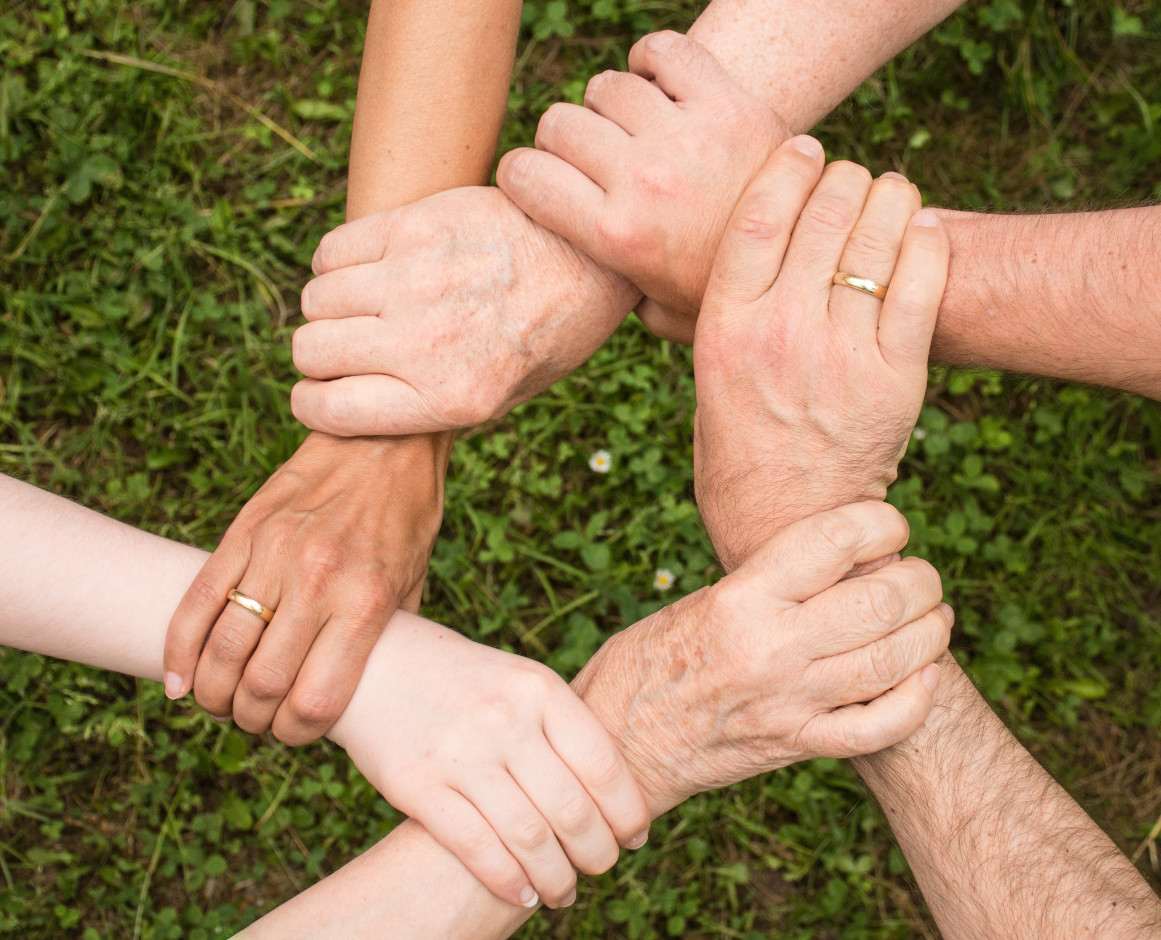
\includegraphics[height=2.8cm]{ground-group-growth-461049}
\includegraphics[height=2.8cm]{accomplishment-ceremony-college-267885}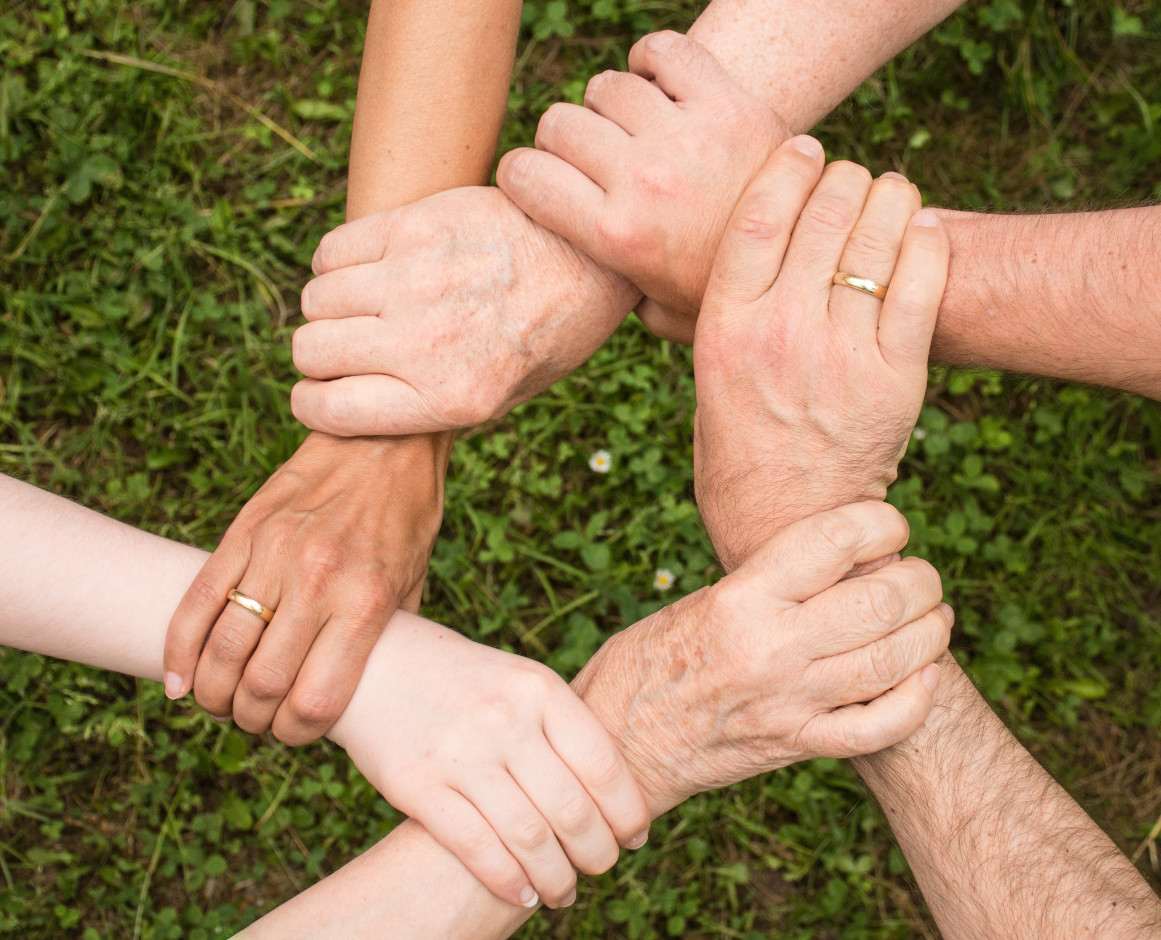
\includegraphics[height=2.8cm]{ground-group-growth-461049}
\includegraphics[height=2.8cm]{blur-book-stack-books-2}}


\begin{document}

\begin{frame}[plain]{}
	\maketitle
\end{frame}


\section{Motivation}
\begin{frame}{Challenges for HPC (and Open Source) Training}
		\begin{itemize}
			\item Not all users possess the right level of training
				\begin{itemize}
				\item Inefficient usage of systems, frustration, lost potential
				\item Good training saves compute time and costs!
				\end{itemize}
      \item Diverse user background and goals
        \begin{itemize}
          \item Science is the goal, HPC is the vehicle
          \item Need to run an application to complete the PhD
        \end{itemize}
      \item Learning is not easy
			\begin{itemize}
				\item Users need to understand beneficial knowledge for tasks
				\item There exist various different training material
				\item Teaching of different data centers is hard to compare
			\end{itemize}
			\item Data center have difficulties to verify the skills of users
      \item Confusion of trainers and HPC practitioners regarding skills
        \begin{itemize}
          \item What should one person know/train regarding "MPI"?
        \end{itemize}
		\end{itemize}
\end{frame}

\begin{frame}{The 
\includegraphics[width=0.45\textwidth]{hpccf-full}}
		\begin{block}{Goals}
			\begin{itemize}
				\item Fine-grained HPC knowledge representation $\Rightarrow$ Competence Standard
          \begin{itemize}
            \item What competences exist, how are they defined?
            \item Puzzle of competences for everyone (practitioners, students, admins)
            \item Supporting navigation and role-specific knowledge maps
          \end{itemize}
				\item Establishing international certificates attesting knowledge
        \item Supporting an ecosystem around the HPC competences
			\end{itemize}
		\end{block}

    \begin{block}{Scope of the forum}
    \begin{itemize}
      \item Central authority for competence representation, certification, and support
      \item Purposeful limitations of the forum:
			\begin{itemize}
				\item We do not compete with content providers
				\item We do not create a curriculum (university/centers responsibility)
			\end{itemize}
    \end{itemize}
		\end{block}
\end{frame}


\begin{frame}{The 
\includegraphics[width=0.45\textwidth]{hpccf-full}}

	\begin{block}{Organization Details}
		\begin{itemize}
			\item Started in 2018 as a spin-off from a project
      \item An independent international body
			\item Organized into
				\begin{itemize}
					\item Steering board (elected)
					\item Full members (with voting rights) - Contributors
					\item Associate members (anyone and any institution)
          \item Collaboration with e.g., SIGHPC Education Chapter
				\end{itemize}
		\end{itemize}
	\end{block}

	\begin{block}{Activities}
		\begin{itemize}
			\item Curating and maintaining the \textbf{Competence Standard}
			\item Providing tools and ecosystem around the competences
		\end{itemize}
	\end{block}
\end{frame}





\begin{frame}{Governance}
	\smallskip
  Various processes are documented \hrefb{https://www.hpc-certification.org/processes/}{here}.
  \begin{block}{Steering Board}
  \vspace*{-0.5em}
  \begin{itemize}
    \item General chair: Julian Kunkel (University of Göttingen / GWDG)
    \item Skill-tree curator: Kai Himstedt (University of Hamburg)
    \item Topic curators:
    \begin{itemize}
      \item HPC Knowledge: Lev Lafayette (University of Melbourne)
      \item Performance Engineering: Anja Gerbes (Technische Universität Dresden)
      \item Sofware Development: Marc-Andre Hermanns (RWTH Aachen)
      \item Administration: Sudeep Narayan Banerjee (Indian Institute of Technology Gandhinagar)
    \end{itemize}    
  %  \item Examination curator: Christian Meesters (University of Mainz)
    \item Publicity chair: Weronika Filinger (University of Edinburgh)
    \item Other topics are jointly managed by the board
  \end{itemize}
  \end{block}
\end{frame}



\begin{frame}{Organization}
  \begin{block}{Organization of the members}
	\begin{itemize}
  \item Webpage is the central hub (\url{https://www.hpc-certification.org})
  \item Mailinglists (news, members, board)
	\item Monthly public meetings on our Slack channel
  \item Monthly meeting of the board
  \item Annual general assembly (BoF at ISC or independent workshop)
  \end{itemize}
  \end{block}

  \begin{block}{Data handling}
    \begin{itemize}
      \item Everything* is developed/available in the open \\
        GitHub (\url{https://github.com/HPC-certification-forum})
      \item Exception are examination questions
    \end{itemize}
  \end{block}
\end{frame}












\begin{frame}[plain]{Motivation}
TU Dresden
\begin{itemize}
 \item[--] is a member of the National High Performance Computing (NHR) since January 2021. (\small{\url{https://tu-dresden.de/zih/hochleistungsrechnen/nhr-center}})
 \item[--] defined several competences in their NHR application.
 %\begin{itemize}
 % \item Performance Analysis and Optimization / Performance Engineering
 % \item Innovative Storage Architecture
 % \item Machine Learning
 % \item Big Data \& High Performance Data Analytics
 %\end{itemize}

 \item[--] started their NHR Training Sessions in September 2021. (\small{\url{https://tu-dresden.de/zih/hochleistungsrechnen/nhr-training}}) 
\end{itemize}

\end{frame}

{\usebackgroundtemplate{%
%  \tikz[overlay,remember picture] 
%  \node[opacity=0.3, at=(current page.south east),anchor=south east,inner sep=0pt] {
%    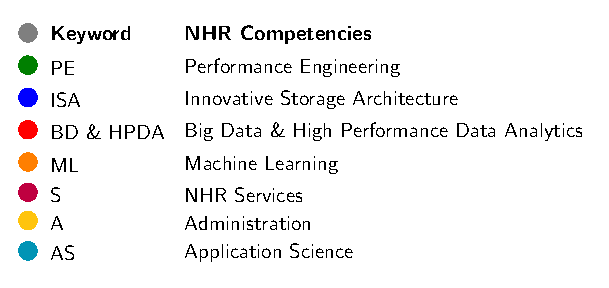
\includegraphics[width=0.70\textwidth]{zih_schwerpunkte.pdf}
%}
%    \hspace*{\sidebarwidth}
%\begin{picture}(100,100)
%\end{picture}
\put(295,-95){
    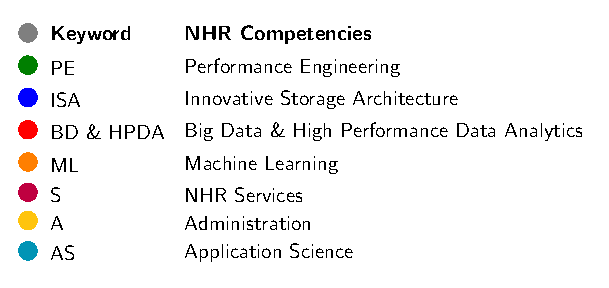
\includegraphics[width=0.40\textwidth]{zih_schwerpunkte.pdf}
    }

\put(0,-245){
   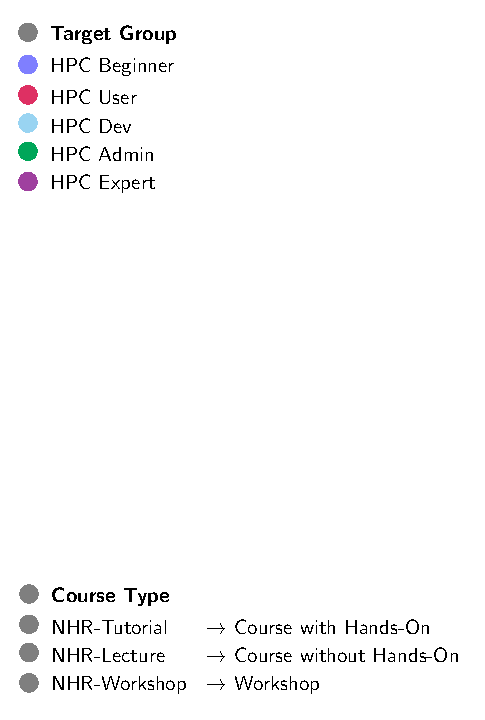
\includegraphics[width=0.35\textwidth]{definition.pdf}
    }
}
\begin{frame}{NHR Training-Portfolio 2023 @ ZIH}
\vspace{-0.3cm}
\begin{center}
 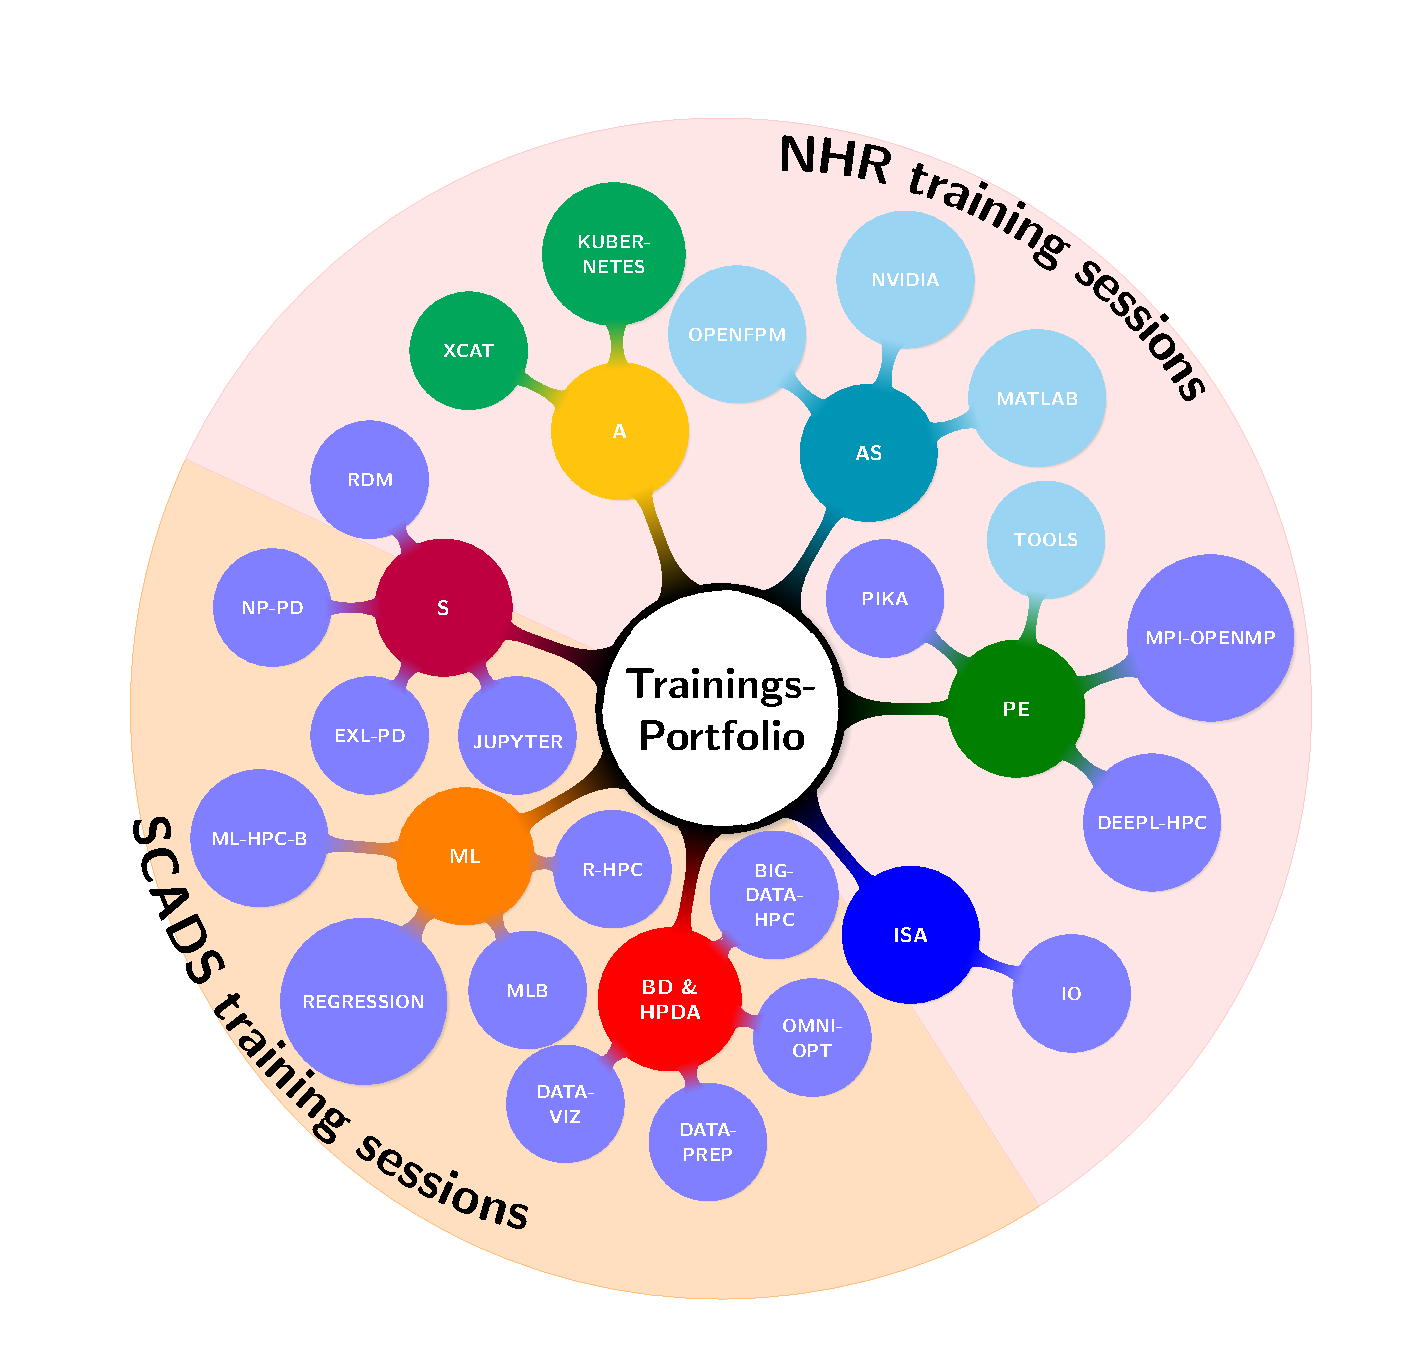
\includegraphics[width=0.55\textwidth]{mindmap_23_plot_nhr_scads_20230503.pdf} 
\end{center}

\end{frame}
}


\section{Strategy}
\sectionIntroHidden

\begin{frame}{Classification of Competences == Skills}
	\begin{itemize}
		\item A \textbf{skill} defines background, objectives, learning outcomes
		\item The \textbf{skill tree} organizes the competences as hierarchical skills
		\item Certificates bundle several skills into attestable unit
	\end{itemize}

	\begin{figure}
		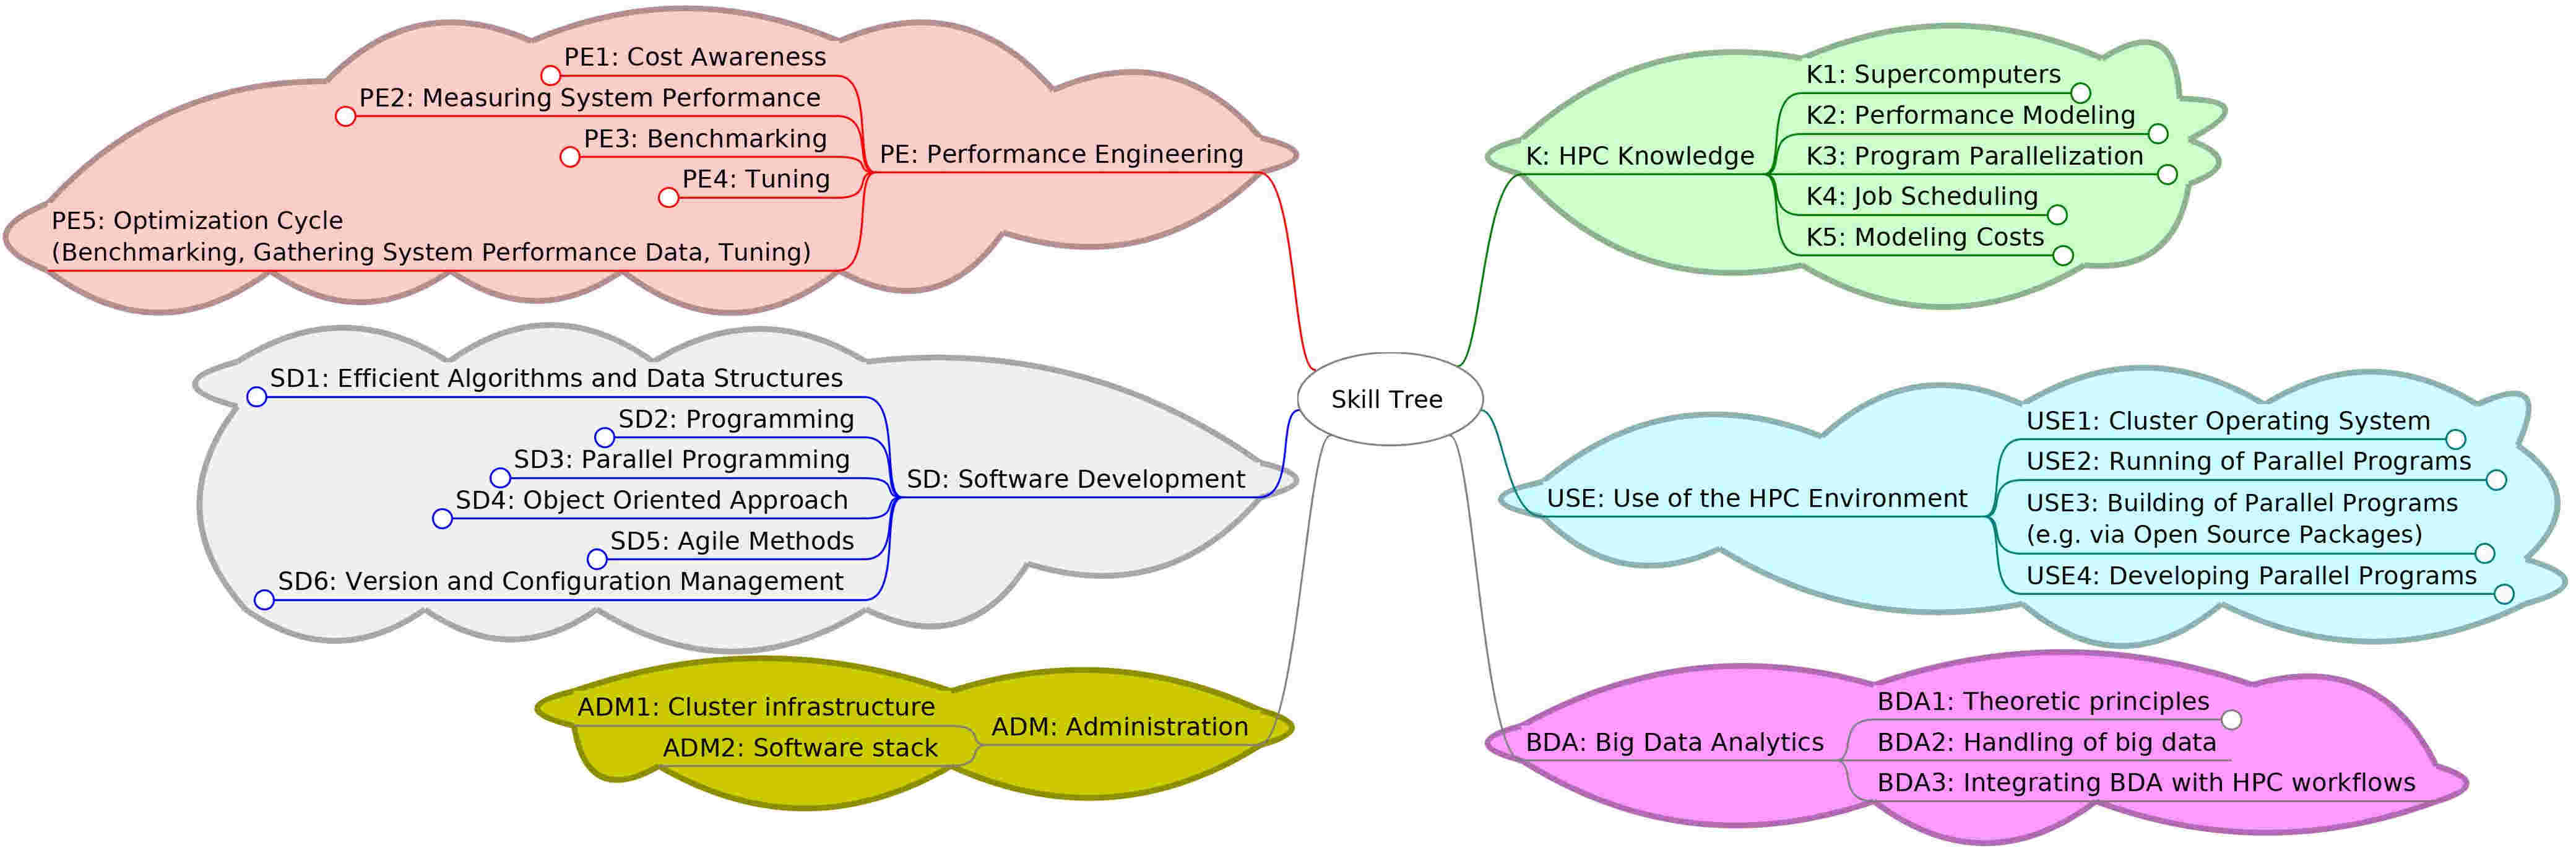
\includegraphics[width=\textwidth]{skill-tree}
		\vspace*{-2em}
		\caption{Top-levels of the skill tree (Initial ADM and BDA branches)}
	\end{figure}
\end{frame}

\begin{frame}{Example High-Level Skill (Excerpt)}
\begin{itemize}
\item Name: Command Line Interface
\item Id: USE1.1-B
\item Background: {\small HPC systems are usually accessed via a Linux-based Command Line Interface (CLI) that is provided by a shell.
At its core, a shell is ...}
\item Aim:
\begin{itemize}
\item describe the key principles of a shell
\item execute basic programs to query system information and manipulate...
\end{itemize}
\end{itemize}

\begin{block}{Learning outcomes (these must be examinable)}
\begin{itemize}
\item Utilize the bash shell to execute individual programs with arguments
\item Describe the meaning of the exit code of a program
\item Run multiple programs after another depending on the exit code ;, \&\&, ||
\item List the set of basic programs and their tasks:
\begin{itemize}
  \item pwd
  \item ... See \url{https://www.hpc-certification.org/wiki/skill-tree/use/1/1/b}
\end{itemize}
\end{itemize}
\end{block}
\end{frame}

\begin{frame}{Classification of HPC Competences}
	\begin{itemize}
		\item Granularity of skill descriptions
		\begin{itemize}
			\item Too fine $\Rightarrow$ content of a skill is predefined at leaf level
			\item Too coarse $\Rightarrow$ no help for structuring the material
			\item Guiding principle: leaf node should be covered in 1-4 hour lecture/workshop
		\end{itemize}


    \item Organization of HPC skills
    \begin{itemize}
      \item Skills are typically depending on sub-skills $\Rightarrow$ tree structure
      \item References to skills are possible; still skills are building blocks for various tasks
      \item One skill can have multiple instances for different skill levels (basic, ..., expert)
    \end{itemize}


    \item Verification of skill tree and certification approach
      \begin{itemize}
        \item Feedback by the HPC community/practitioners justify the approaches
      \end{itemize}
	\end{itemize}
\end{frame}




\begin{frame}{Contribution to the Skill-Tree High-Level Editing}

  \begin{block}{How can members contribute?}
  \begin{itemize}
    \item Webpage with Markdown version controlled in Git
      \begin{itemize}
        \item \url{https://www.hpc-certification.org/wiki/skill-tree/b}
        \item GitHub: \url{https://github.com/HPC-certification-forum/skill-tree}
        \begin{itemize}
          \item Pull requests, reviews, comments, ...
        \end{itemize}
      \end{itemize}
    \item Editing a MindMap, the structure of Skills
      \begin{itemize}
        \item Synchronized with the skill tree in Git
        \item Uses the OpenSource tool Freemind
      \end{itemize}
    \item Discussion on our \href{https://join.slack.com/t/hpc-certification/shared_invite/enQtMzUwNzU3NzM2MTkzLTAzZWM3NDg0N2I2ZmQwOWI5ZGUwNjNlNDgzM2RmOTM3ZWRjNjIxYTc5NzUxYTJhNmRlNmM5YmE1NDY3YzkzYzA}{Slack}
    \item Documented in our \hrefb{https://www.hpc-certification.org/processes/}{processes section}
    \item See our videos on \href{https://www.youtube.com/playlist?list=PL4b682pSp7MQbdhhvwisrPo7PjYya26_g}{YouTube}
    \item Visit us and join our Slack/mailing lists: \url{https://hpc-certification.org}
  \end{itemize}
  \end{block}
\end{frame}


\begin{frame}{NHR Training-Portfolio 2023 @ ZIH}
%\framesubtitle{Needed Steps}
{
\footnotesize
\begin{columns}[T]
\hspace{1.25cm} \begin{column}{0.55\textwidth}
Speaker:
\begin{itemize}[itemsep=0pt]
 \item[--] Define Course Type
 \item[--] Define Target Group
 \item[--] Define Course Title
 \item[--] Write Summary 
 \item[--] Define Agenda
 \item[--] Create Reference Guide (optional)
 \item[--] Define Questions for Survey
 \item[--] Define Prerequisites  \textbf{\textcolor{red}{$\longrightarrow$ $\longrightarrow$ $\longrightarrow$ \hspace{0.01cm} \rotatebox[origin=b]{270}{$\Rsh$} }}
 \item[--] Define Learning Objectives \textbf{\textcolor{red}{$\longrightarrow$ \rotatebox[origin=b]{270}{$\Rsh$} \hspace{0.13cm} $\downarrow$ }}  
 \end{itemize}
\vspace{-0.1cm}
\hspace{3.25cm} \textbf{\textcolor{red}{mapping $\downarrow$ \hspace{0.10cm}  $\downarrow$} }
\vspace{-0.1cm}
 
\begin{itemize}
 \item[--] Search/Define HPC-CF Skill Tree Entry
\vspace{-0.2cm}
 \begin{itemize}
  \item[--] {\footnotesize Background }
  \item[--] {\footnotesize Aim }
  \item[--] {\footnotesize Outcomes }
 \end{itemize}

\end{itemize}
\end{column}
\begin{column}{0.55\textwidth}
NHR Coordinator:
\begin{itemize}[itemsep=0pt]
 \item[--] Define Questions for Survey 
 \item[--] Create Course Website Link
 \item[--] Create Registration Link
 \item[--] Create Survey Link
 \item[--] Create Certificate of Participation
\end{itemize}
%\vspace{1.5cm}
%\begin{itemize}
% \item Search/Define HPC-CF Skill Tree Entry
% \begin{itemize}
%  \item Background
%  \item Aim
%  \item Outcomes
% \end{itemize}
%\end{itemize}
\end{column}

\end{columns}
}
\end{frame}


\begin{frame}{HPC-CF Skills point of view}
\vspace*{-0.9cm}
%\begin{center}
 
% 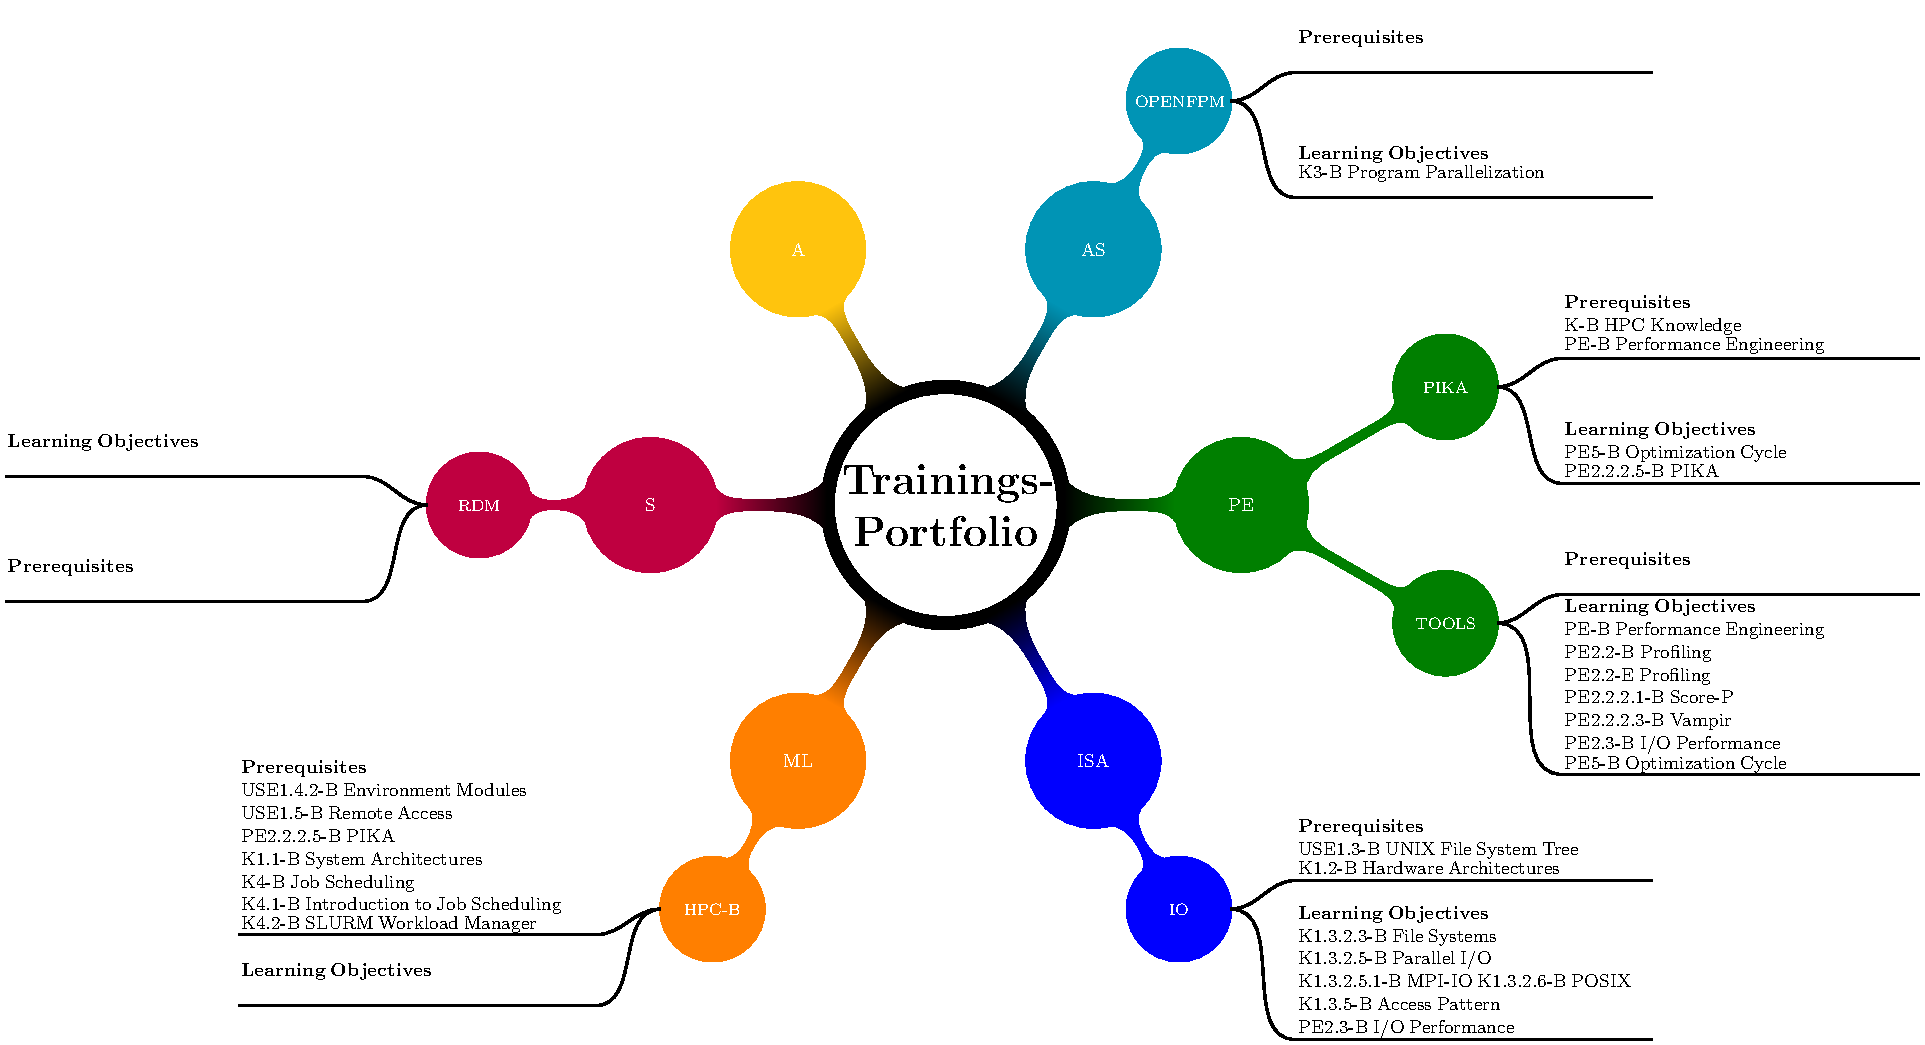
\includegraphics[width=1.15\textwidth]{zih_automate_14122021.pdf} 
%\end{center}
 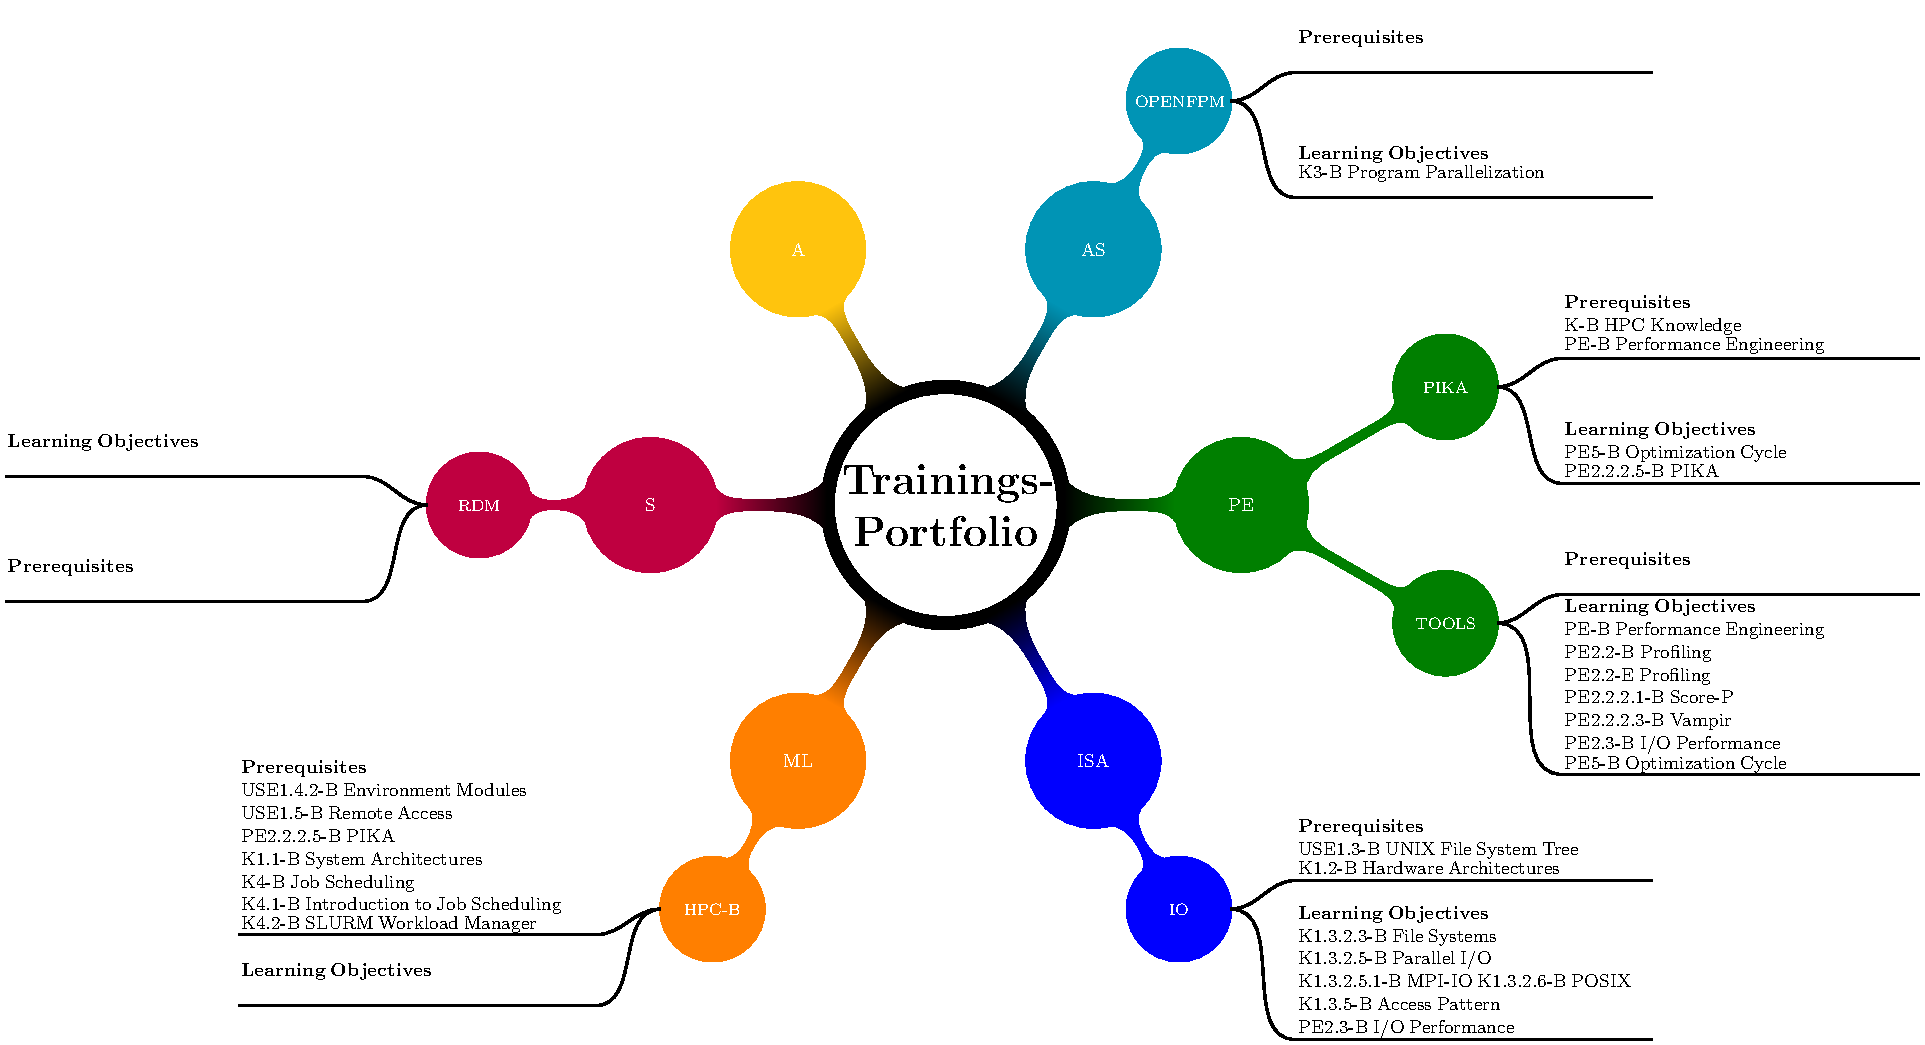
\includegraphics[width=1.05\textwidth]{zih_automate_14122021.pdf} 

\end{frame}


\begin{frame}{HPC-CF Skill Tree}
\hspace{2.5cm}
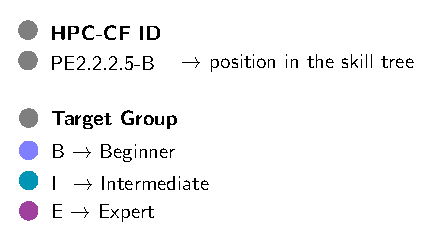
\includegraphics[width=0.35\textwidth]{definition_skills.pdf}
   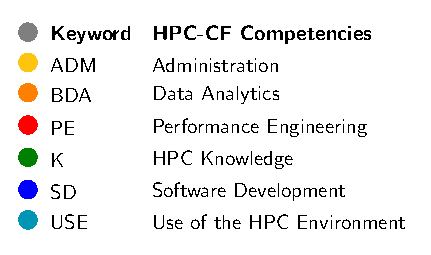
\includegraphics[width=0.40\textwidth]{hpccf_schwerpunkte.pdf}
\vspace{1.5cm}
    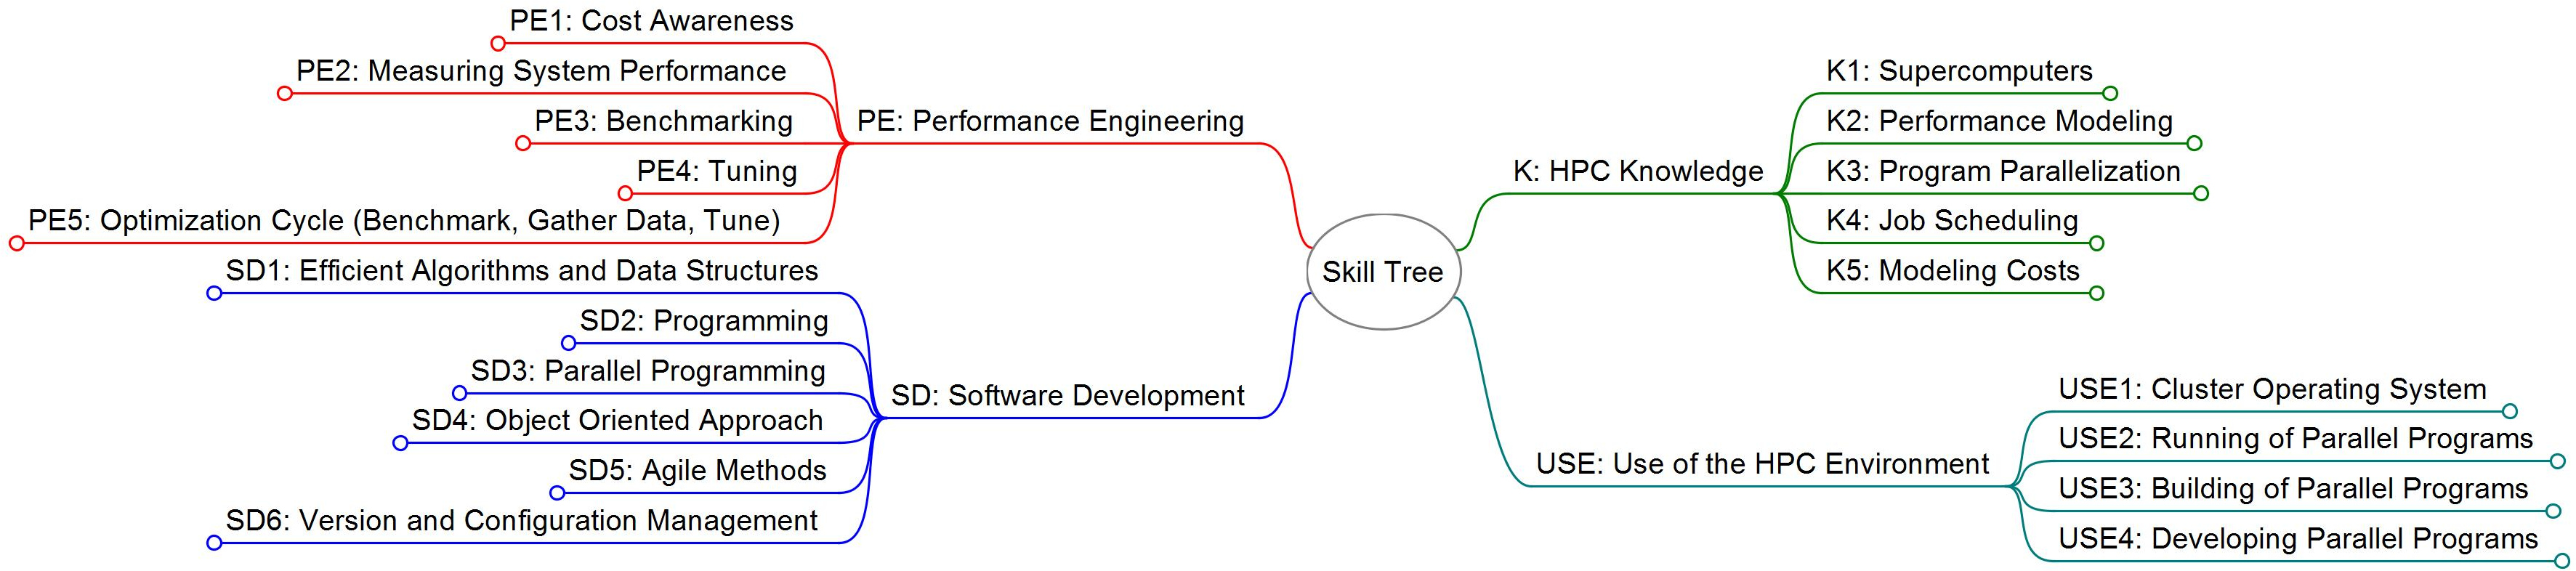
\includegraphics[width=1.00\textwidth]{skill-tree_top_levels.jpg}

\end{frame}


\begin{frame}
\frametitle{HPCCF Skills of NHR Trainings}
   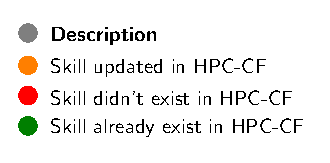
\includegraphics[width=0.25\textwidth]{hpccf_skills.pdf}
   \\
   \url{https://www.hpc-certification.org/wiki/skill-tree/b}
\begin{columns}[T]
\begin{column}{0.5\textwidth}
\begin{itemize}[itemsep=0pt]
 \item[--] \textcolor{green!50!black}{PE5-B Optimization Cycle} 
 \item[--] \textcolor{red}{PE2.2.2.5-B PIKA}
\item[--]  \textcolor{orange}{K1.3.2.3-B File Systems}
\item[--] \textcolor{orange}{K1.3.2.5-B Parallel I/O}
\item[--] \textcolor{green!50!black}{K1.3.2.5.1-B MPI-IO}
\item[--] \textcolor{orange}{K1.3.2.6-B POSIX}
\item[--]  \textcolor{orange}{K1.3.5-B Access Pattern}
 \item[--] \textcolor{green!50!black}{PE-B Performance Engineering}
\end{itemize}
\end{column}
\hspace{-0.5cm}
\begin{column}{0.65\textwidth}
\begin{itemize}[itemsep=0pt]
 \item[--] \textcolor{green!50!black}{PE2.2-B Profiling}
 \item[--] \textcolor{orange}{PE2.3-B I/O Performance}
 \item[--] \textcolor{orange}{PE2.3-I I/O Performance}
 \item[--] \textcolor{green!50!black}{PE2.2-E Profiling}
 \item[--] \textcolor{green!50!black}{ PE5-B Optimization Cycle}
 \item[--] \textcolor{red}{PE2.2.2.1-B Score-P}
 \item[--] \textcolor{red}{PE2.2.2.3-B Vampir}
\end{itemize}
\end{column}

\end{columns}
\end{frame}


%\section{Certification Process}
%\sectionIntroHidden



\end{document}
